\chapter{Ergebnisse}

In diesem Kapitel wird die implementierte Lauferkennung ausgewertet und es werden ebenfalls die Ergebnisse der Testversuche vorgestellt und diskutiert.

Die Auswertung der Versuche beziehungsweise der Testergebnisse wird aus zeitlichen Gründen qualitativ aber nicht quantitativ sein.


\section{Verifizierungsversuche}

Die bereits im \autoref{ab:Versuchsplanung} aufgelisteten Versuchsszenarien wurden alle mindestens einmal getestet. Einige Testszenarien wurden in zwei Testdurchläufen durchgeführt.
Nach der Durchführung der Verifizierungsversuche werden die Ergebnisse analysiert und diskutiert. 

Die Lauferkennung ist ein großer Teil dieser Arbeit und wird demnächst mit den tatsächlichen Daten (Ground Truth) sowie der von Google integrierte Aktivitäts\-erkennung verglichen.
\section{Lauferkennung}

In der \autoref{fig:Speed_Groundtruth_MotionClass_GoogleMD_Compare} werden die verschiedenen Methoden der Aktivitätserkennung sowie die Geschwindigkeit in der obersten Grafik über die Zeit dargestellt.

Die zweite Grafik zeigt die tatsächliche Aktivitätsdaten (Ground Truth), die in vier Klassen (\autoref{fig:Lauferkennung_Klassentabelle}) unterteilt sind. Die Aktivitätsbereiche sind mit vertikalen roten Linien optisch unterteilt, die auch in anderer Grafiken sichtbar sind, damit diese einfach und schnell zugeordnet werden können. 

Bei der Sekunde \SI{460}{\second} sowie \SI{500}{\second} ist die Versuchsperson vom Motorrad ab- oder aufgestiegen, deswegen werden diese zwei Stellen mit \glqq No Motion\grqq{} klassifiziert. Ab der Sekunde \SI{556}{\second} gibt es keine Videoaufnahme mehr und es wurde \glqq Undefined\grqq{} eingetragen.

In der dritten Grafik ist die Ausgabe der im Rahmen dieser Arbeit implementierten Lauferkennung beziehungsweise Aktivitätserkennung abgebildet. 
Es ist zu bemerken, dass die Lauferkennung eine sehr große Übereinstimmung mit der Ground Truth hat. Laufen sowie Fahren werden dadurch gut erkannt. Das Auf- und Absteigen bei den Sekunden \SI{465}{\second} und \SI{508}{\second} wird der \glqq No Motion\grqq{}-Klasse vom Lauferkennung-Modell zugeordnet.

Die letzte Grafik stellt die Ausgabe der im Smartphone integrierten Aktivitäts\-erkenn\-ung dar, die für diese Auswertung in die gleiche Klassifizierung aus der \autoref{fig:Lauferkennung_Klassentabelle} umgerechnet wird.
%\begin{landscape}
%	\centering
	\begin{figure}[htpb]
		\centering
%		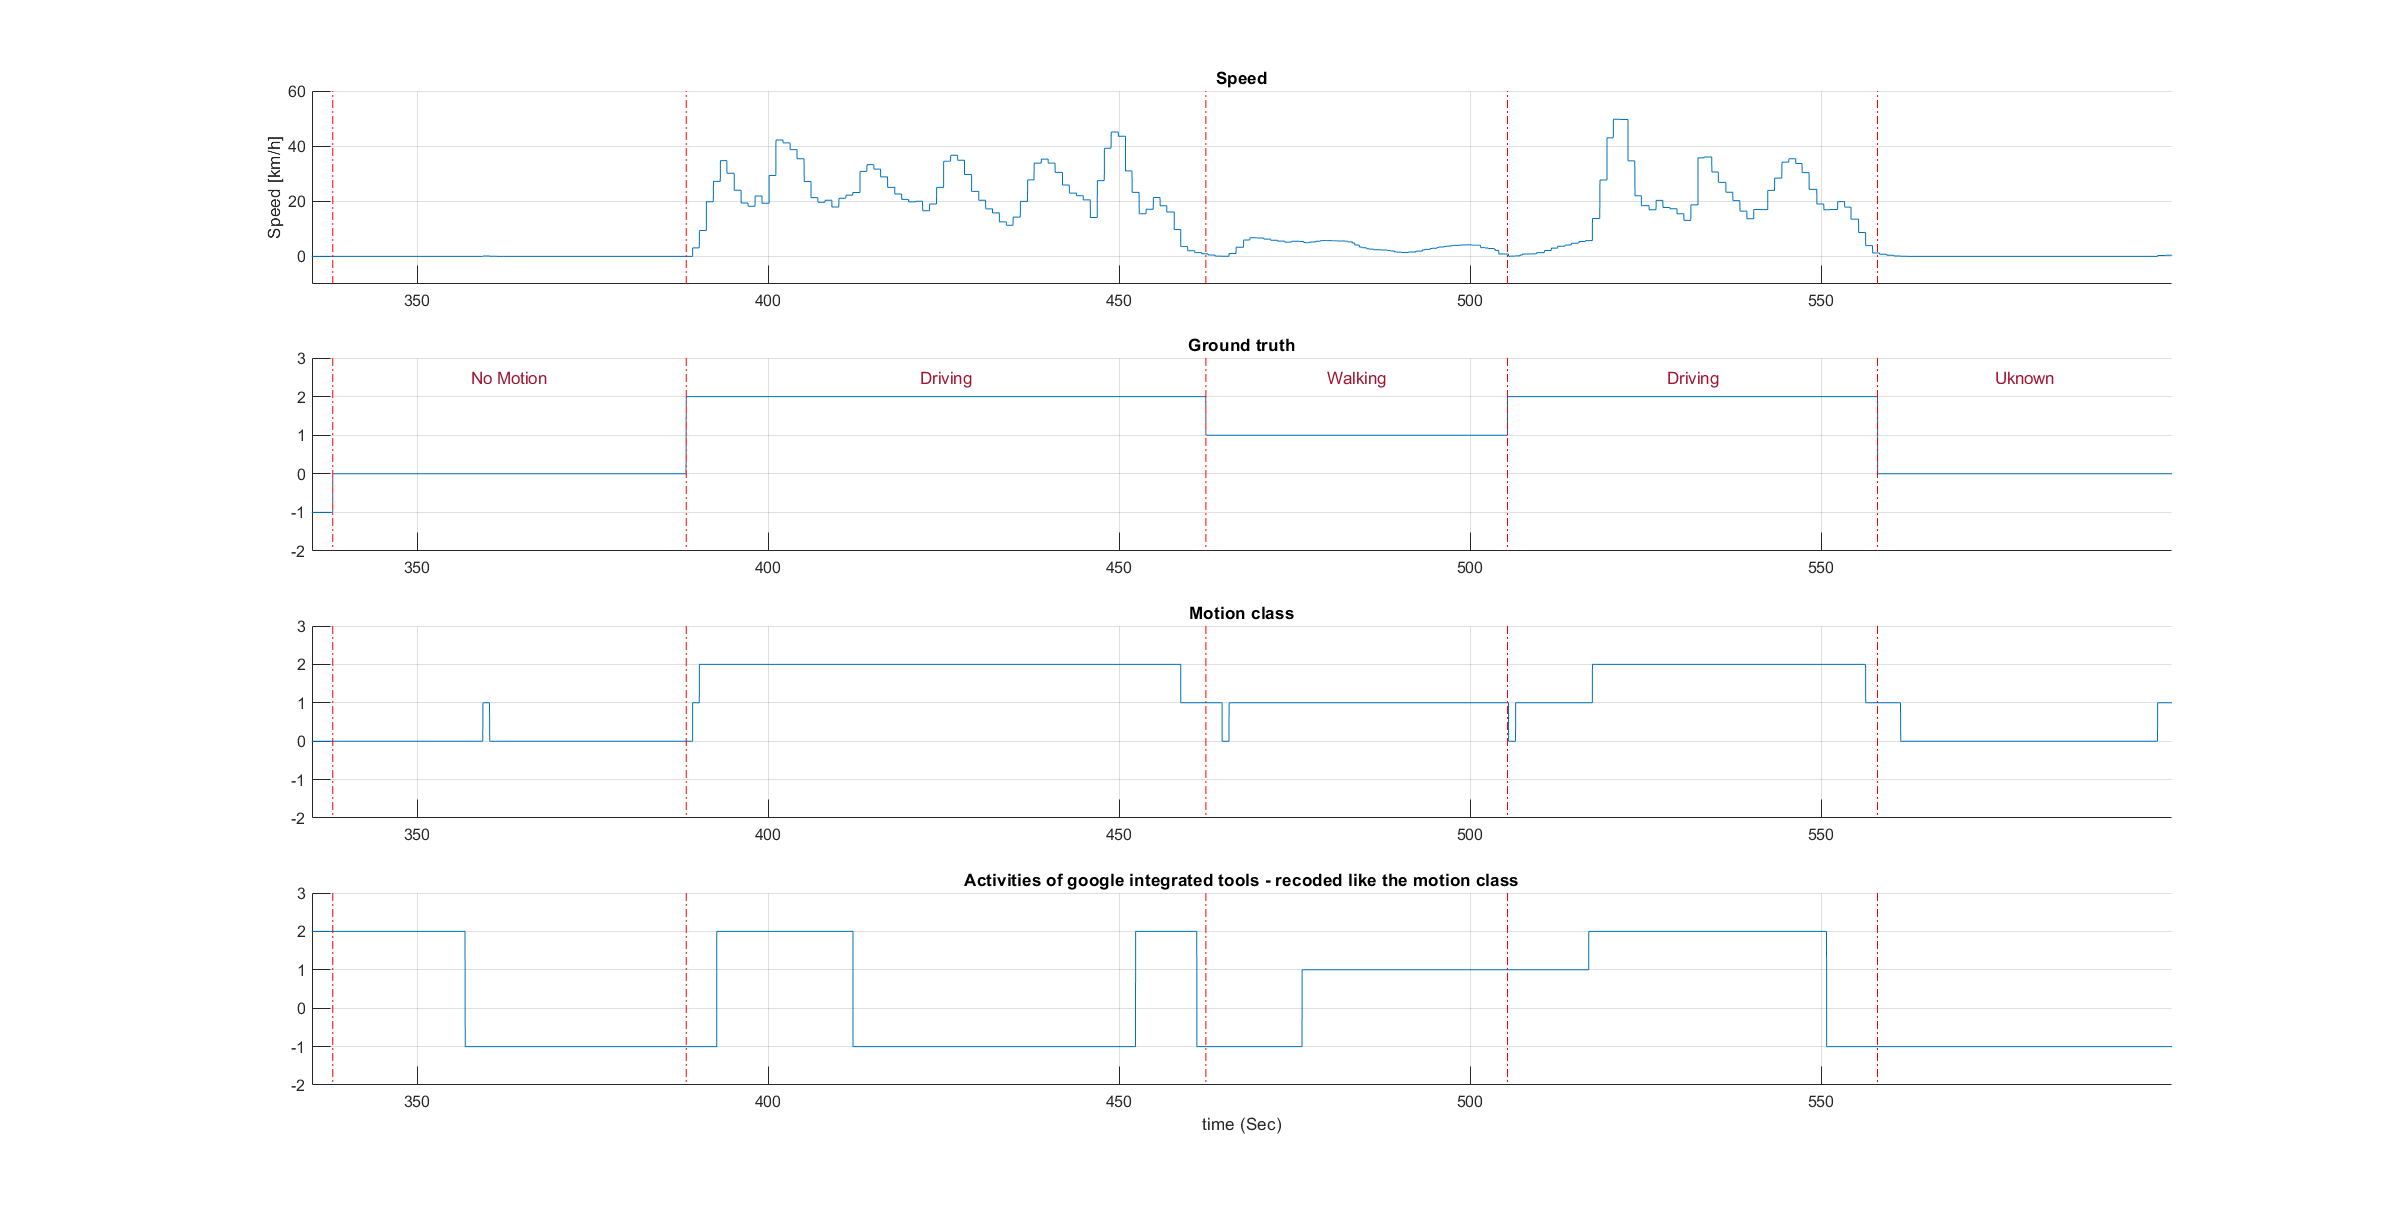
\includegraphics[width=\textwidth]{Bilder/Speed_Groundtruth_MotionClass_GoogleMD_Compare.png}
		\psfragfig[width=\textwidth]{Bilder/0B_WalkingDet_Compare}
		\caption{Ergebnis des Lauferkennungsmodells}
		\label{fig:Speed_Groundtruth_MotionClass_GoogleMD_Compare}
	\end{figure}
%\end{landscape}
%\begin{figure} % TODO: Tabelle machen
%	\centering
%	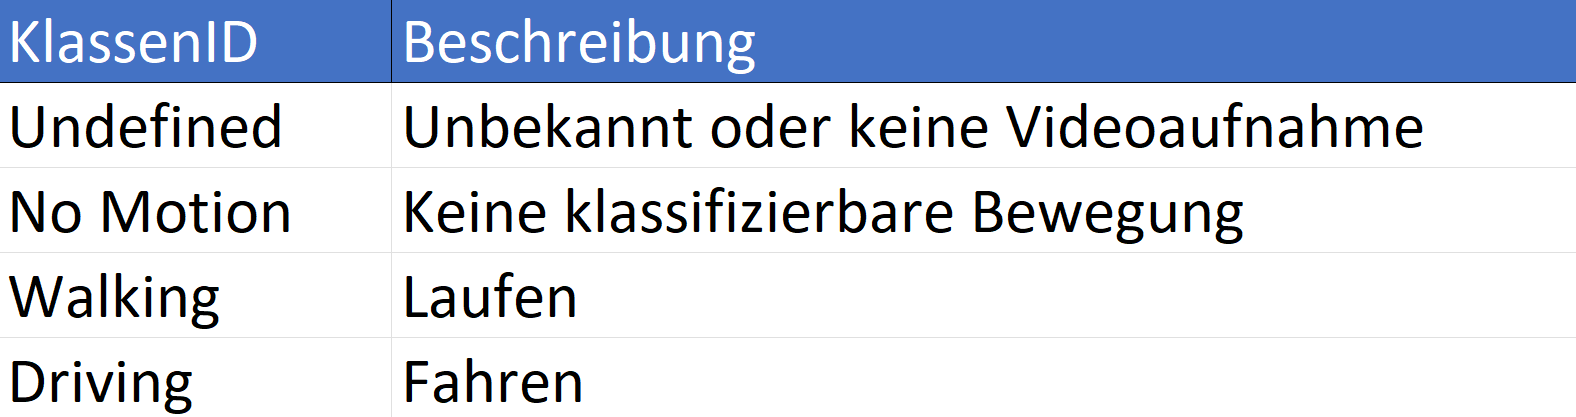
\includegraphics[width=0.6\linewidth]{Bilder/Lauferkennung_Klassentabelle.png}
%	\caption{Beschreibung der Klassen in der Grafik \autoref{fig:Speed_Groundtruth_MotionClass_GoogleMD_Compare}}
%	\label{fig:Lauferkennung_Klassentabelle}
%\end{figure}


Aus der \autoref{fig:Speed_Groundtruth_MotionClass_GoogleMD_Compare} ist letztendlich zu erkennen, dass die Aktivitäts\-erkenn\-ung durch das implementierte Modell gute Ergebnisse liefert, die mit der Wahrheit sehr gut übereinstimmen. Im Vergleich zu der Google-Aktivitäts\-erkenn\-ung (unterste Grafik) hat das Modell eine wesentlich bessere Aussage getroffen. Die implementierte Aktivitätserkennung verbraucht keine große Rechenzeit (ca. $2$ bis $3$ Sekunden) und erfolgt in Echtzeit mit einer kleinen Verzögerung (ca. \SI{2,5}{\second}), da die FFT erst durchführbar ist, wenn \SI{256}{Messwerte} vorhanden sind.

\begin{table}[htpb]
	\caption{Beschreibung der Klassen in der \autoref{fig:Speed_Groundtruth_MotionClass_GoogleMD_Compare}}
	\label{fig:Lauferkennung_Klassentabelle}
	\centering
	\begin{tabular}{|l|l|}
		\hline
		\textbf{Klasse} & \textbf{Beschreibung}\\
		\hline
		Undefined & Unbekannt oder keine Videoaufnahme\\ 
		\hline
		No Motion &  Keine klassifizierbare Bewegung\\ 
		\hline
		Walking & Laufen\\ 
		\hline
		Driving & Fahren\\ 
		\hline
	\end{tabular}
\end{table}

\section{Verschiedene Fahrerpositionierung}
\begin{figure}[htpb]
	\centering
	%	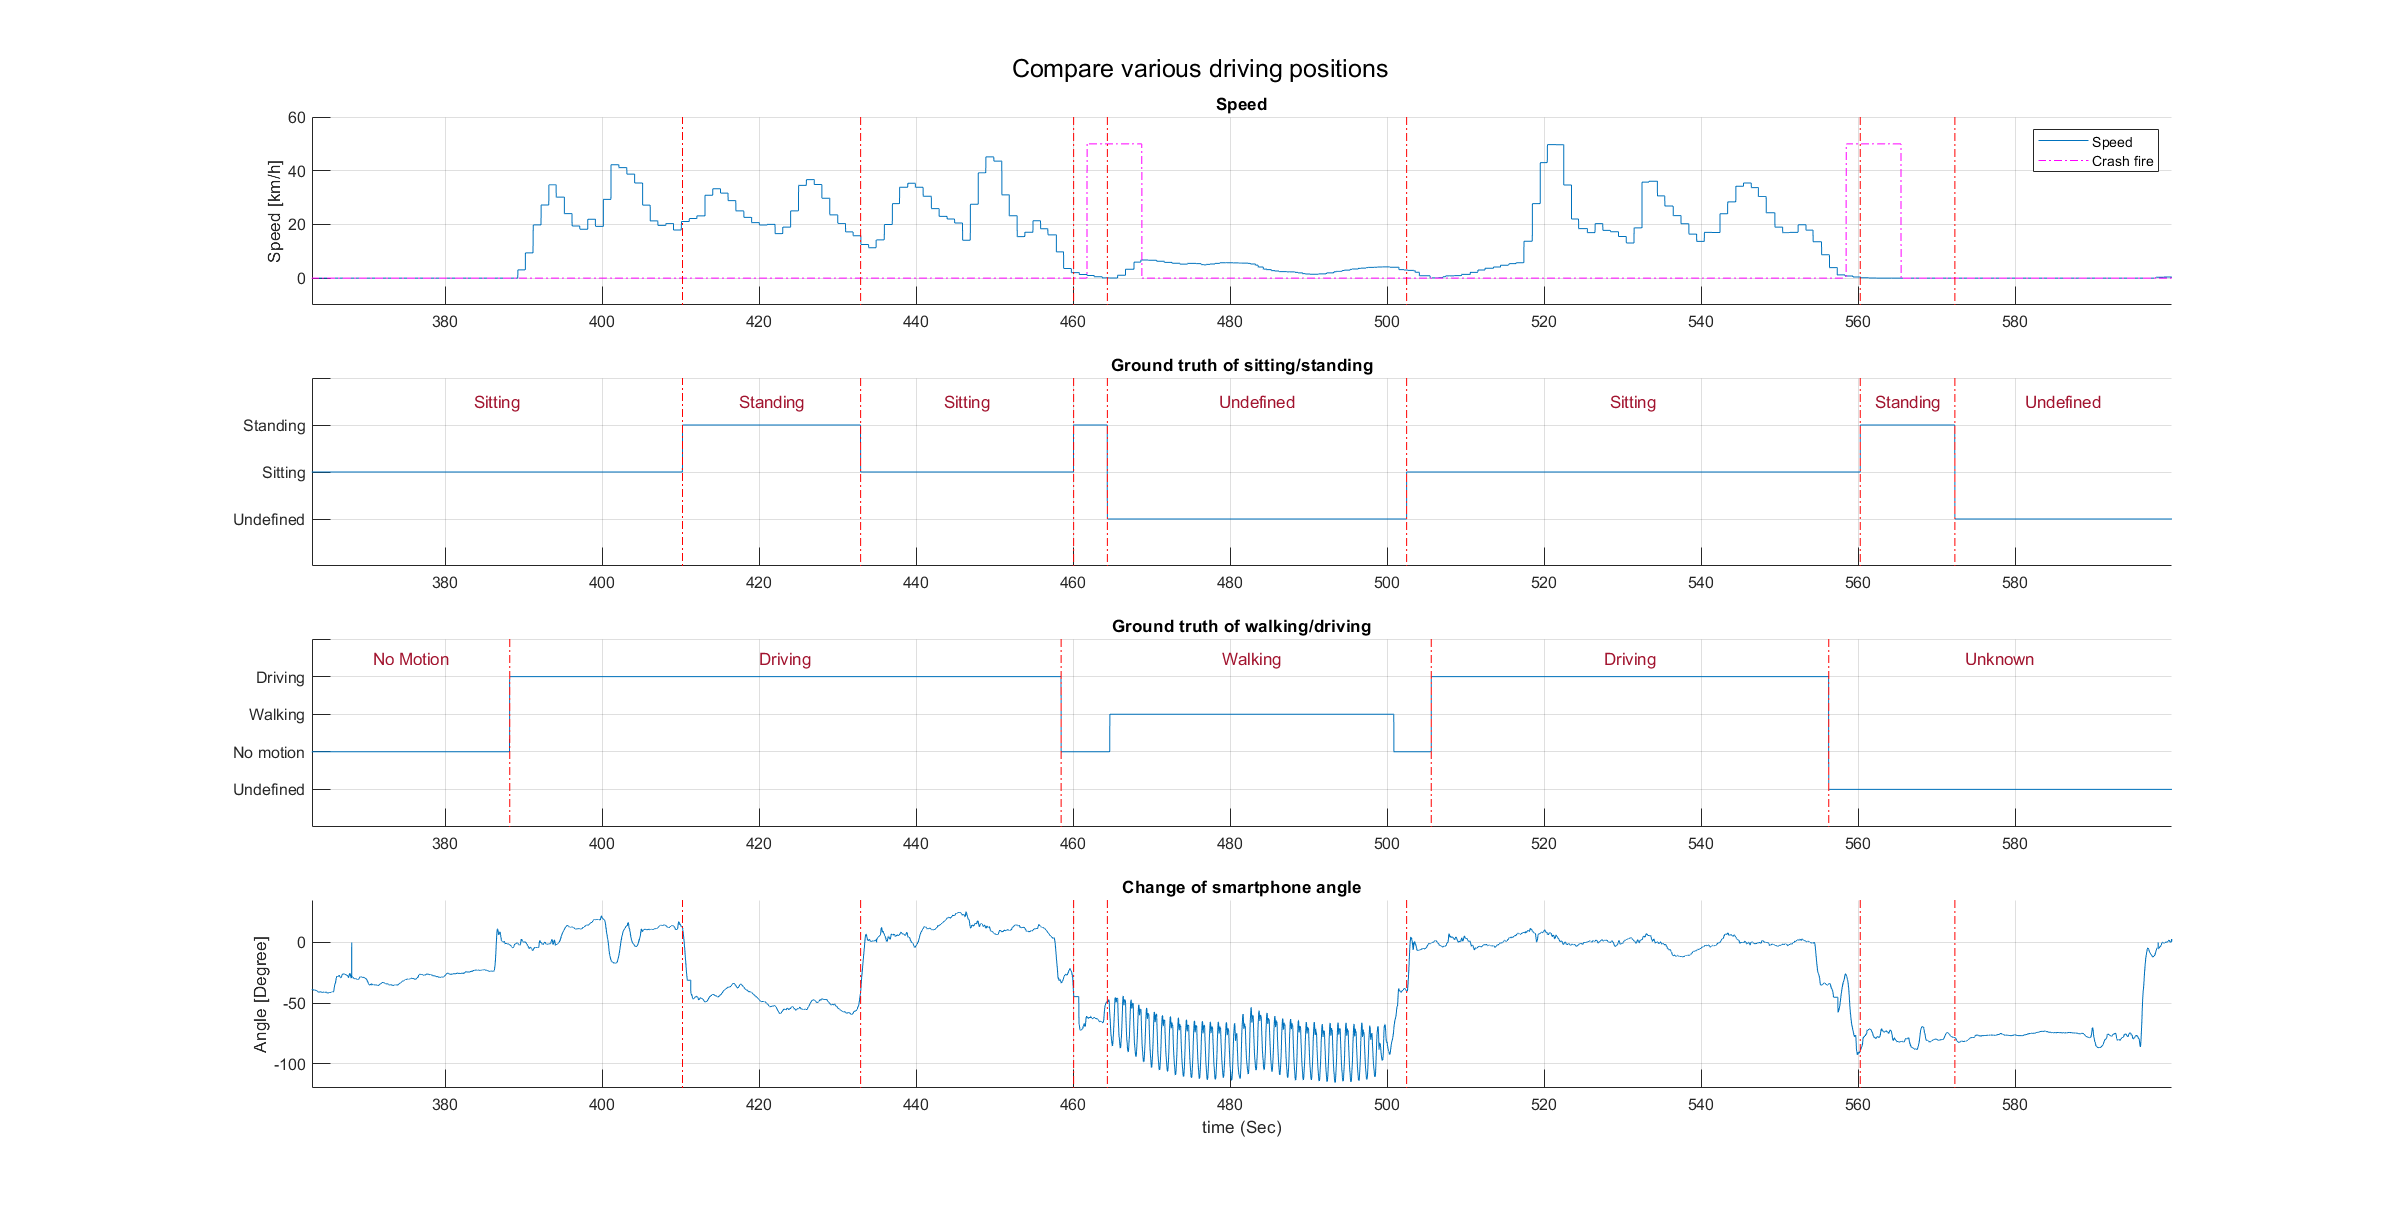
\includegraphics[width=\linewidth]{Bilder/Speed_Groundtruth_WalkStand_Compare.png}
	\psfragfig[width=\textwidth]{Bilder/0B_CompareDrivingPos}
	\caption{Zeitlicher Verlauf der Geschwindigkeit, Ground Truth der Fahreraktivität und -Position sowie der Winkeländerung}
	\label{fig:Speed_Groundtruth_WalkStand_Compare}
\end{figure}
Die \autoref{fig:Speed_Groundtruth_WalkStand_Compare} dient zur Auswertung des ersten Testszenarios aus der \autoref{tab:TestSzenarienZusammenfassung}, in dem die Person während einer Fahrt auf der Fußraste des Motorrads für paar Sekunden steht und sich wieder setzt. Das Ziel dieses Tests ist zu prüfen, ob die Änderung der Fahrerposition während einer Fahrt zur falschen Alarmauslösung führt.

Diese Darstellung zeigt die Geschwindigkeit, die Fahreraktivität (Fahren/Laufen), die Fahrerposition sowie die Winkeländerung über die Zeit.

Die Geschwindigkeit (blau) sowie die Alarmauslösungen während der Fahrt (lila) sind in der ersten Grafik abgebildet.
Die zweite Grafik stellt die tatsächliche Fahrerposition (Ground Truth) über die Zeit dar, die in drei Klassen (Sitzen, Stehen oder unbekannt) unterteilt ist.
Die Fahrerpositionsbereiche sind ebenfalls durch vertikale rote Linien optisch geteilt, die auch in den anderen Grafiken sichtbar sind, damit diese einfach und schnell zugeordnet werden können.
In dem Zeitbereich zwischen \SI{465}{\second} und \SI{505}{\second} ist die Versuchsperson gelaufen, deswegen lautet die Klassifizierung \glqq Unbekannt\grqq{}, da die geplante Klassen einen solchen Fall nicht abdecken.

In der dritten Grafik sind die tatsächliche Aktivitätsdaten (Ground Truth) darstellt, die in vier Klassen (\autoref{fig:Lauferkennung_Klassentabelle}) unterteilt sind. Die Aktivitätsbereiche sind auch mit vertikalen roten Linien optisch unterteilt. Beim Betrachten der zweiten und dritten Grafik lässt sich ein guter Überblick über die Fahrt verschaffen. Zwischen den Sekunden \SI{388}{\second} und \SI{459}{\second} fand eine Fahrt statt, während dieser hat der Fahrer zwischen den Sekunden \SI{410}{\second} und \SI{433}{\second} gestanden.

Die Kurve aus der letzten Grafik zeigt die Winkeländerung des Smartphones im Vergleich zur ursprünglichen Position nach der Kalibrierung. Aus der Darstellung ist die Winkeländerung während der ersten Fahrt, als die Fahrerposition sich verändert hat, sehr gut sichtbar. Das Laufmuster ist in diesem Signal zwischen \SI{465}{\second} und \SI{500}{\second} ebenfalls gut erkennbar.
%\begin{landscape}

%\end{landscape}


Es ist wichtig zu bemerken, dass die Änderung der Fahrerposition während einer Fahrt keine Fehlalarme (die lila Kurve aus der obersten Grafik) ausgelöst hat, da die Winkeländerung in so einem Fall nicht groß genug ist, um das \glqq TipOver\grqq{}-Model zu aktivieren. Beim Absteigen (ca. \SI{460}{\second} und \SI{560}{\second}) gibt es allerdings eine Alarmauslösung, da es an der Stelle eine sehr große Winkeländerung gibt, da der Fahrer sein Bein nach außen und hinten gestreckt hat.
\section{Anhalten}
Dieser Abschnitt diskutiert das Ergebnis des zweiten Testszenarios aus der \autoref{tab:TestSzenarienZusammenfassung}, in dem die Versuchsperson während einer Fahrt kurz anhält und seinen Fuß auf den Boden herunter setzt.

\begin{figure}[htpb]
	\centering
	\psfragfig[width=\linewidth]{Bilder/0B_Anglechanging_stopping}
	\caption{Winkeländerung des Smartphones durch das Anhalten}
	\label{fig:Speed_AngleChangeCompare}
\end{figure}
Die Grafik \autoref{fig:Speed_AngleChangeCompare} zeigt die Geschwindigkeit sowie die Winkeländerung zur ursprünglichen Position nach der Kalibrierung über die Zeit.
Während des Tests ist zu sehen, dass der Fahrer dreimal anhält und seinen Fuß herunter setzt, was in der Geschwindigkeitskurve sichtbar ist (\SI{262}{\second}, \SI{315}{\second} und \SI{350}{\second}). Es wurde während des Tests entgegen den Erwartungen keine Fehlalarmauslösung gegeben. Nach einer genaueren Analyse ist der Grund bekannt worden.

Die Winkeländerung beträgt nicht \ang{90} sondern nur ca. \ang{20}-\ang{30} (\autoref{fig:MotorbikeDrivingStanding}). Die Person hat ihr Bein beim Sitzen nicht genau horizontal sondern leicht nach unten geneigt. Wenn der Fahrer sein Fuß herunter setzt, ist diese ebenfalls nicht genau vertikal sondern leicht geneigt mit einem Winkel von ca. \ang{10}-\ang{20} zur Vertikalen . Daher ist die Winkeländerung nicht über \ang{45} und sollte auch zu keinen Alarmauslösungen führen.

\begin{figure}[htpb]
	\centering
	\begin{subfigure}{0.48\textwidth}
		\centering
		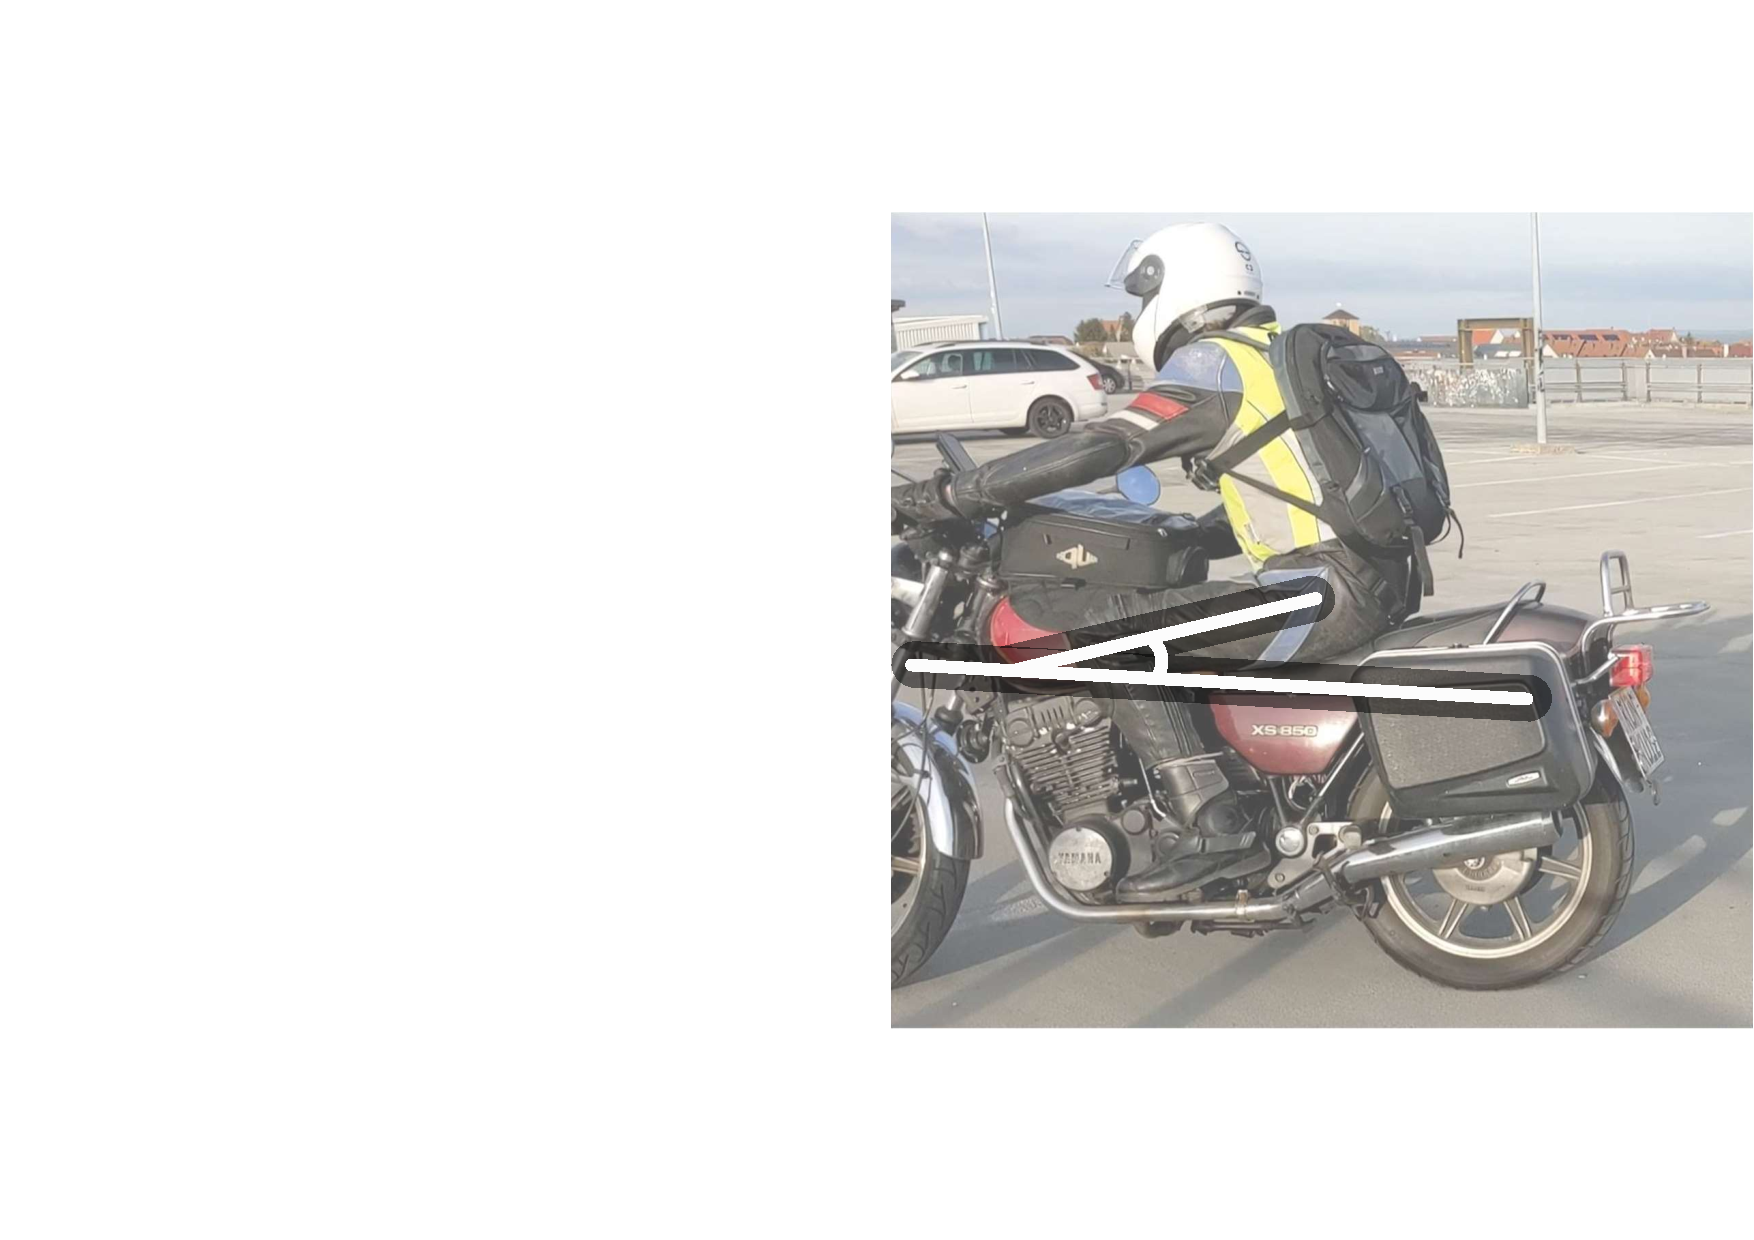
\includegraphics[width=\textwidth]{Bilder/0_Beinposition_Anhalten_Fahren.pdf}
		\caption{Beinposition während einer Fahrt}
		\label{fig:MotorbikeDriving}
	\end{subfigure}
	\hfill
	\begin{subfigure}{0.48\textwidth}
		\centering
		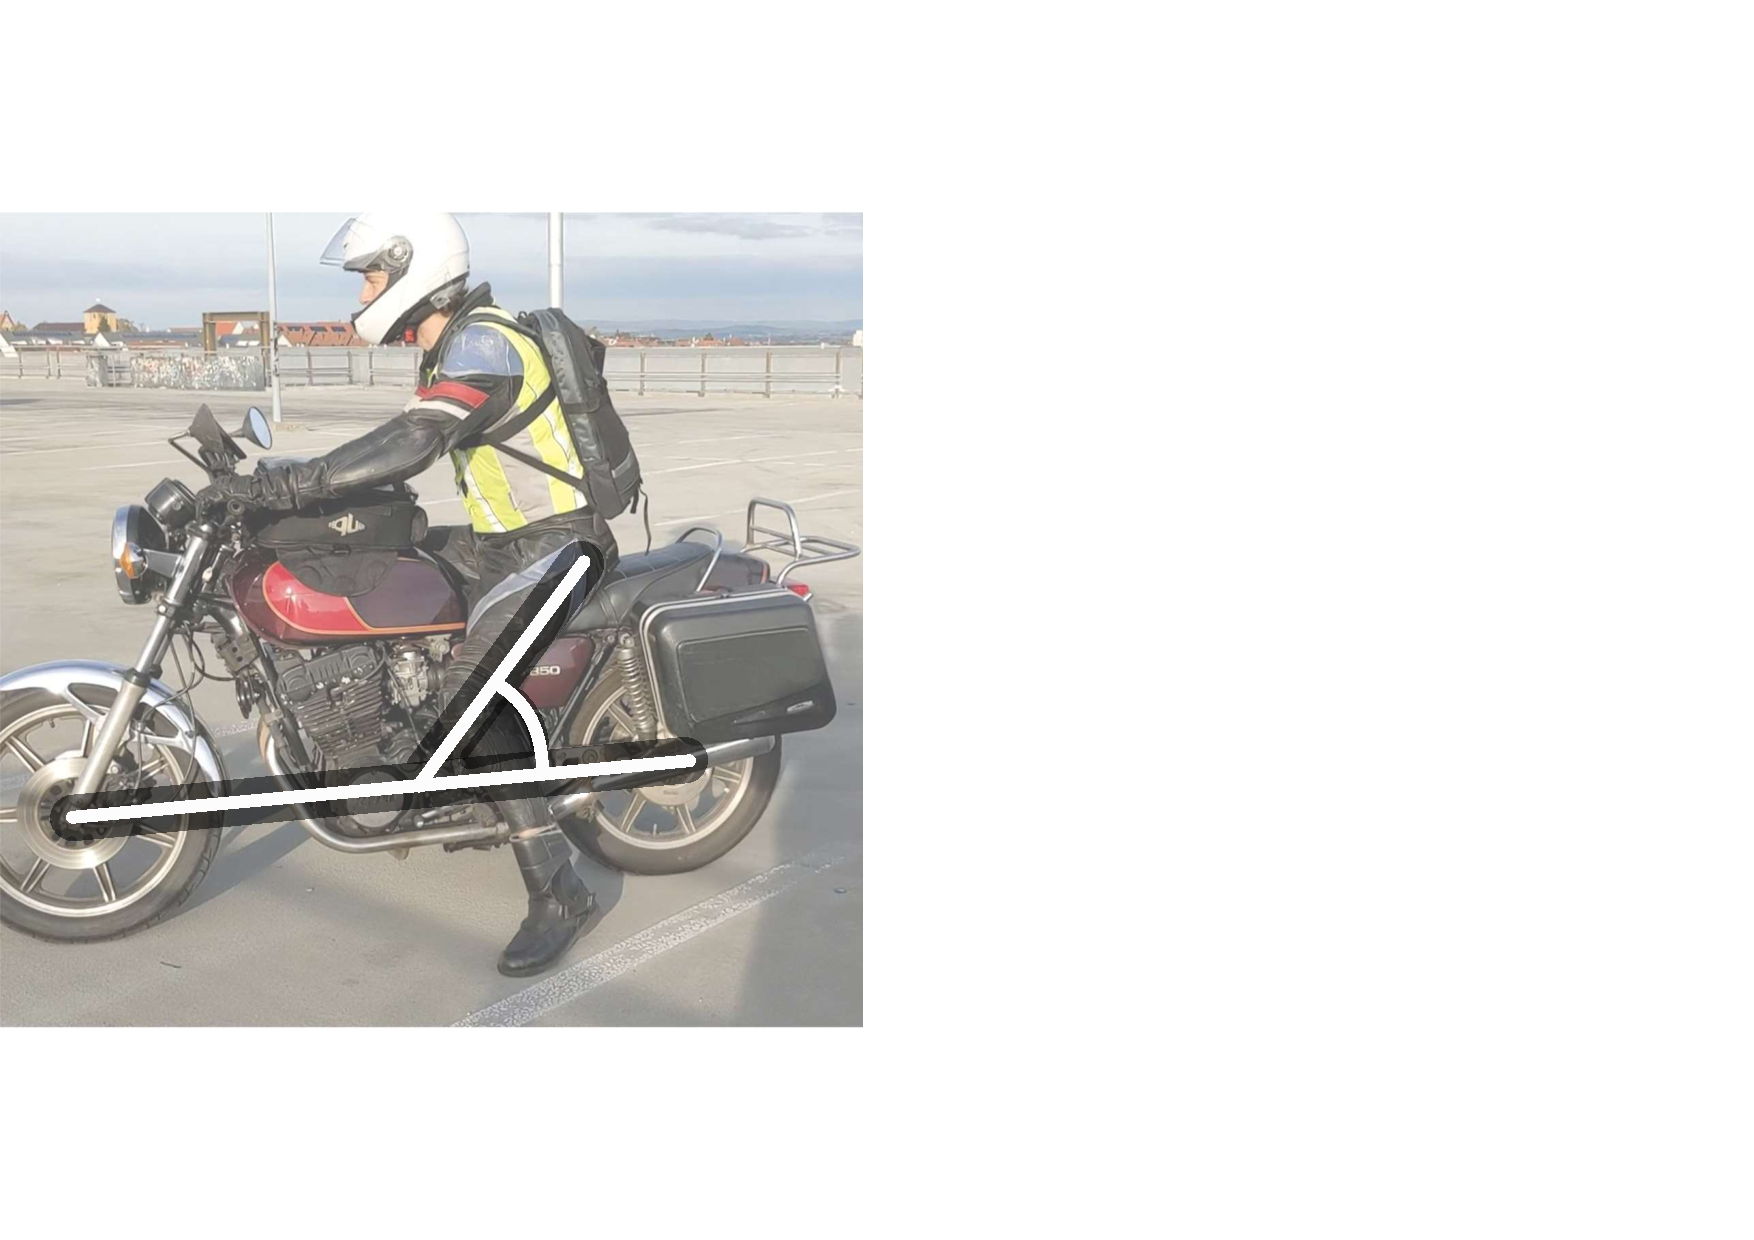
\includegraphics[width=\textwidth]{Bilder/0_Beinposition_Anhalten_Stehen.pdf}
		\caption{Beinposition Beim Anhalten}
		\label{fig:MotorbikeStanding2}
	\end{subfigure}
	\caption{Beinpositionen während einer Fahrt und beim Anhalten}
	\label{fig:MotorbikeDrivingStanding}
\end{figure}


 